%! Author = Frederik Bußmann
%! Date = 22.06.2023

\section{Fachlicher Hintergrund} \label{sec:02-background}

Für die Erarbeitung einer geeigneten \acrshort{ci}-Strategie wird zunächst ein Einblick in die Disziplin des
Continuous-Software-Engineering gegeben.
Anschließend werden die Begrifflichkeiten und Prinzipien von Continuous Integration definiert.
Darüber hinaus wird eine Übersicht über die Funktionen und Mechanismen der Shopware-Plattform gegeben.

\subsection{Continuous Software Engineering} \label{subsec:02-background-1}

Continuous-Software-Engineering fasst die Prinzipien der Continuous Integration (\acrshort{ci}),
Continuous Delivery (\acrshort{cde}), und Continuous Deployment (\acrshort{cd}) zusammen.
Shahin et al.\ definieren den Begriff als einen Bereich der Softwareentwicklung, bei dem es um die Entwicklung,
Auslieferung und das schnelle Feedback von Software und Kunde geht.
Die Disziplin umfasst Geschäftsstrategie und Planung, sowie Entwicklung und den Betrieb der Software.
\footpartcite[3910--3911]{tools-and-practises}
Diese kontinuierliche Integrierung von Software ist sehr kompatibel mit den häufigen iterationen in der agilen
Softwareentwicklung und wurde unter anderem durch die agile Methodik des Extreme Programming bekannt.
\footpartcite{fitzgerald}
Nachfolgend werden die Bereiche der agilen Softwareentwicklung und der \acrshort{ci}, \acrshort{cde} und \acrshort{cd}
kurz erläutert.

\subsubsection{Agile Software Development}

Agile Softwareentwicklung ist ein Ansatz zur Softwareentwicklung, der auf Flexibilität und Kundeninteraktion setzt.
Im Gegensatz zu traditionellen, plangetriebenen Methoden, die die Anforderungen und Lösungen am Anfang des Projekts
festlegen, erlaubt die agile Methodik Änderungen und Anpassungen während des gesamten Entwicklungsprozesses.
Dies wird durch iterative Entwicklung und regelmäßiges Feedback erreicht.
Zu den wichtigsten Prinzipien der agilen Softwareentwicklung gehören die kontinuierliche Auslieferung von Software,
Offenheit für sich ändernde Anforderungen und enge Zusammenarbeit zwischen Teams und Entwicklern.
\footpartcite{agile-manifesto}
Gren und Lenberg fassen Agile als die Reaktionsfähigkeit im Hinblick auf sich ständig ändernde Anforderungen
und Umgebungen zusammen.\footpartcite{agile}

\subsubsection{Continuous Integration}

Continuous Integration (\acrshort{ci}) ist ein Softwareentwicklungsprozess, bei dem Entwickler ihre Änderungen
regelmäßig, oft mehrmals täglich, in ein gemeinsames Repository integrieren.
Jede dieser Integrationen wird dann von einem automatisierten Build-System überprüft, um sicherzustellen, dass die
Änderungen mit der bestehenden Codebase kompatibel sind und keine Fehler verursachen.
Dieser Prozess ermöglicht es Teams, Probleme frühzeitig zu erkennen und zu beheben, was die Qualität der Software
verbessert und die Zeit bis zur Auslieferung der Software reduziert.\footpartcite{fowler}

\subsubsection{Continuous Delivery}

Continuous Delivery (\acrshort{cde}) erweitert das Konzept der Continuous Integration, indem es sicherstellt, dass die
Software stetig in einem Zustand ist, der sicher in die Produktionsumgebung ausgerollt werden kann.
Dies wird durch das Einführen von Integrationstests, die die Funktionalität der vollständigen Software inklusive aller
Module testen, erreicht.
Das Ziel von \acrshort{cde} ist es, den Prozess der Softwareauslieferung zu beschleunigen und zuverlässiger zu machen,
indem menschliche Fehler minimiert und schnelles Feedback über Probleme in der Produktionsumgebung ermöglicht wird.
\footpartcite{humble}

\subsubsection{Continuous Deployment}

Continuous Deployment (\acrshort{cd}) ist der nächste Schritt nach Continuous Delivery.
Bei \acrshort{cd} wird jede Änderung, die den automatisierten Testprozess besteht, automatisch in die
Produktionsumgebung eingespielt.\footpartcite[3911]{tools-and-practises}
Dies bedeutet, dass neue Features und Updates mehrmals täglich an die Endbenutzer ausgeliefert werden können, was eine
schnelle Reaktion auf Marktbedingungen und Kundenfeedback ermöglicht.
Es ist jedoch zu beachten, dass \acrshort{cd} eine hohe Reife der Entwicklungsprozesse und Testautomatisierung
erfordert, um die Anzahl der in der Produktionsumgebung aufkommenden Fehler zu minimieren.
Der Zusammenhang zwischen Continuous Integration, Delivery und Deployment wird in Abbildung\ \ref{fig:ci-cde-cd}
aufgezeigt.

\begin{figure}[H]
    \centering
    \centerline{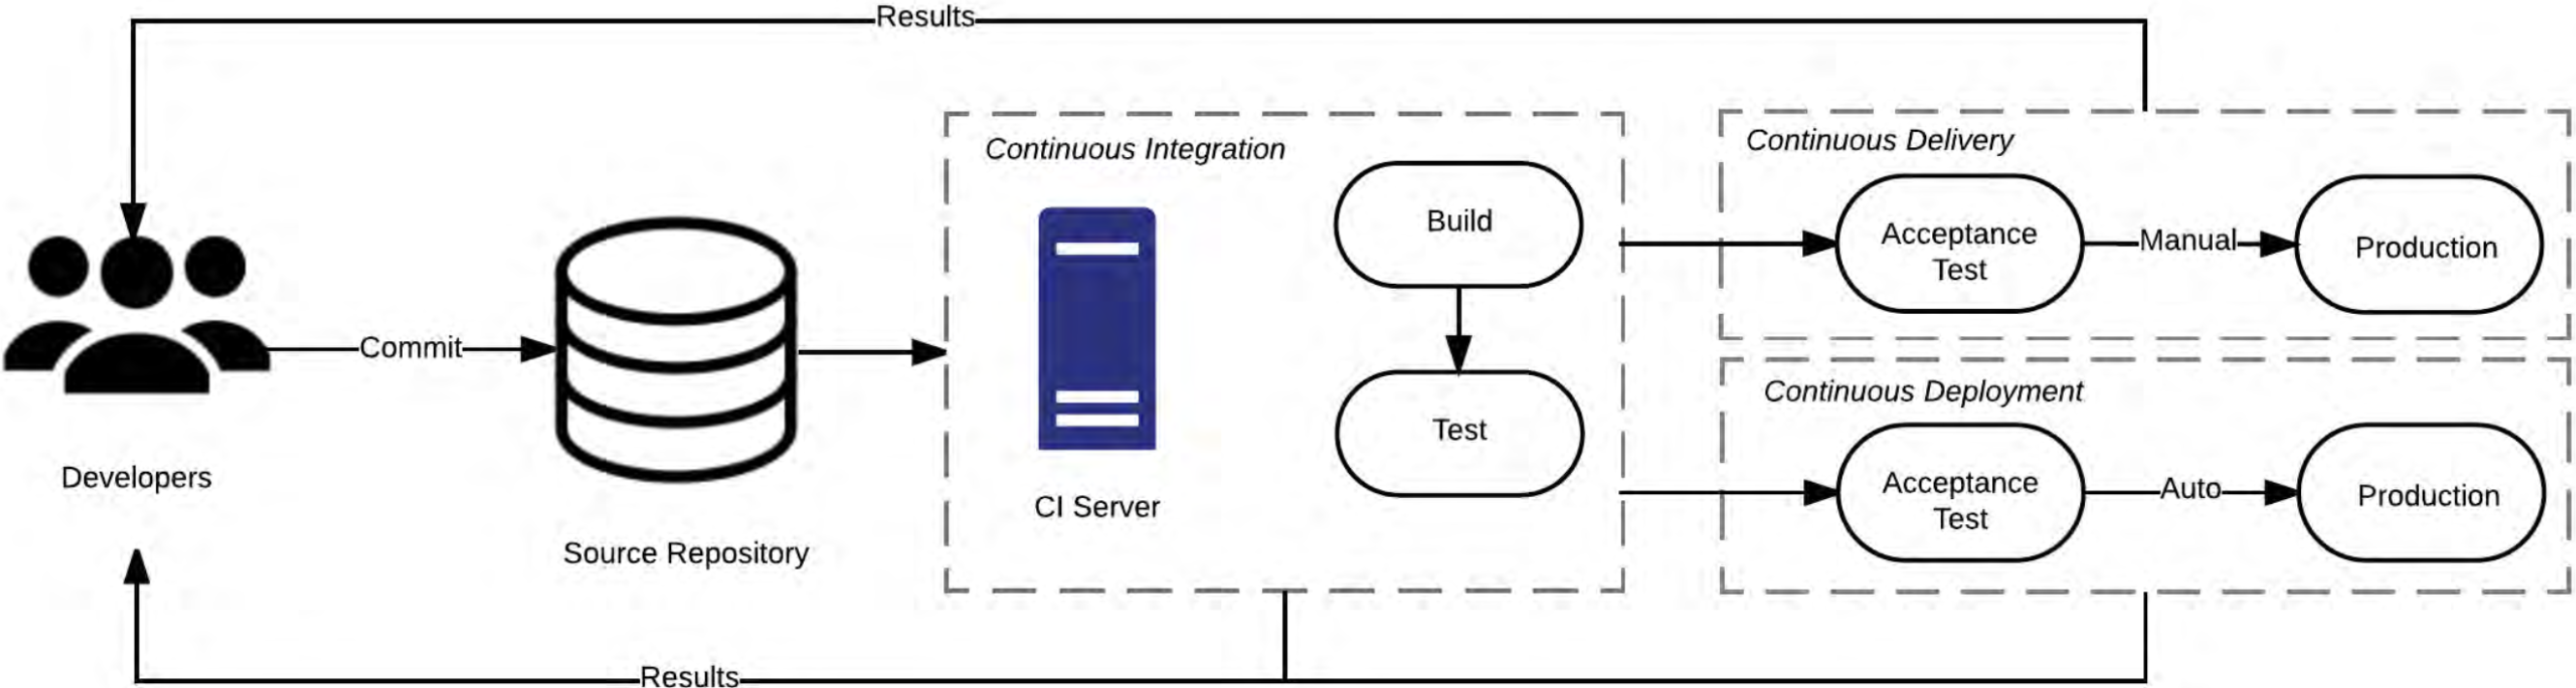
\includegraphics[width=0.91\textwidth]{images/content/ci-cde-cd}}
    \captioncite[Übernommen von]{tools-and-practises}{Zusammenhang zwischen \acrshort{ci}, \acrshort{cde} und \acrshort{cd}}
    \label{fig:ci-cde-cd}
\end{figure}

\subsection{Begrifflichkeiten und Prinzipien von Continuous Integration} \label{subsec:02-background-2}

Um die Bedeutung und den Nutzen von Continuous Integration und des Continuous-Software-Engineering für die
Softwareentwicklung nachvollziehen zu können, ist es hilfreich, einen Blick auf die historische Entwicklung und die
grundlegenden Prinzipien der \acrshort{ci} zu werfen.
Ein Kernprinzip hinter Continuous Integration wurde bereits im Jahr 1991 von Grady Booch definiert.
Hierbei werden Software-Releases nicht als ein großes Ereignis betrachtet, sondern regelmäßig durchgeführt, wobei
die vollständige Software stetig größer wird.\footpartcite{booch}
Kent Beck popularisierte im Jahr 1998 die Disziplin des \glqq Extreme Programming\grqq, wobei großer Wert auf das frühe
und regelmäßige Testen und Integrieren der entwickelten Komponenten einer Software gelegt wird.
Beck behauptet hierbei, dass ein Feature, für welches es keine automatisierten Tests gibt, auch nicht funktioniert.
\footpartcite[2--4]{extreme-programming}
Im Jahr 2006 fasste Software-Entwickler Martin Fowler einige Bereiche dieser Methodiken in dem Artikel
\glqq Continuous Integration\grqq\ unter dem gleichnamigen Begriff zusammen.
Fowler beschreibt \acrshort{ci} als einen Prozess, bei dem Teammitglieder ihre Arbeit regelmäßig Integrieren,
wobei Integration als der Build-Prozess, inklusive automatisierter Tests, für die vollständige Software mitsamt der
erarbeiteten Änderungen zu verstehen ist.\footpartcite{fowler}
Ein Ziel dieser Vorgehensweise ist die Reduktion der \glqq Cycle Time\grqq, welche die Zeitspanne von der Entwicklung
eines Features bis zum Erhalten des Kundenfeedbacks beschreibt.\footpartcite[2580]{benefits-challenges}
Da die erfolgreiche Implementierung von Continuous Integration auf der Kombination von verschiedenen Methoden zur
Verwaltung von Softwareprojekten fußt, werden im Folgenden einige dieser Schlüsselaspekte kurz dargestellt.

\subsubsection{Regelmäßige Integration}

Die namensgebende Methodik der \acrshort{ci} ist das regelmäßige Integrieren von Software und damit Verbunden ist der
Software-Release.
In der traditionellen Softwareentwicklung wird der Release als ein einmaliges, großes Ereignis betrachtet.
Als Integration wird der Prozess des Einbindens einer einzeln entwickelten Komponente in die bisher bestehende
Gesamtheit einer Software bezeichnet, wobei der Release das Zusammenfinden aller Komponenten und das Ausführen des
Build-Prozesses bis hin zur fertigen, ausführbaren und auslieferbaren Software beschreibt.
In der Vergangenheit wurde bei einem Release jede Einzelkomponente der Software manuell integriert und getestet, wobei
dies als eigene Phase in der Entwicklung einer Applikation galt.
In einem \acrshort{ci}-gestützten Projekt wird der Prozess des Software-Releases vollständig automatisiert, sodass jedes
Teammitglied eine entwickelte Komponente schnell Integrieren und einen Software-Build erzeugen kann, was sich positiv
auf die Cycle Time auswirkt.\footpartcite{fowler}
In der Regel finden das Bauen und Testen der Software in einer \glqq Pipeline\grqq\ statt, welche die genutzten
\acrshort{ci}-Tools wie Test-Suites und Static-Code-Analysis ausführt.\footpartcite[2571]{benefits-challenges}

\subsubsection{Automatisierte Tests}

Neben der regelmäßigen Integrierung von Code gelten automatisierte Software-Tests und Quality-Checks als ein wichtiger
Aspekt von \acrshort{ci}.
Hierbei werden oftmals Unit-Tests verwendet, welche eine einzelne Softwarekomponente auf
ihre Funktion prüfen, abgekapselt von anderen Komponenten.\footpartcite[280]{test-driven-development}
Wenn ein Test fehlschlägt, wird in der Regel die Pipeline unterbrochen.
Neben den typischerweise schnell durchlaufenden Unit-Tests, die aufgrund ihrer isolierten Natur spezifische Komponenten
prüfen, können nach dem Build-Prozess umfassende End-To-End-Tests für die gesamte Software durchgeführt werden.
Diese Systemübergreifenden Tests, welche das Zusammenspiel verschiedener Komponenten testen, erhöhen zwar die Dauer des
Test-Prozesses, können aber wichtige Einsicht in die Qualität der Software gewähren.\footpartcite{fowler}
Oftmals kommen auch Static-Code-Analysis Tools zum Einsatz, um eine Pipeline bei Unstimmigkeiten in der Syntax des
eingeführten Codes abzubrechen.\footpartcite[338]{static-analysis}

\subsubsection{Reproduzierbarkeit}

Ein weiterer zentraler Aspekt von Continuous Integration ist die Reproduzierbarkeit der \acrshort{ci}-Pipeline.
In einem \acrshort{ci}-Umfeld werden der Build- und Testing-Prozess vollständig automatisiert und standardisiert, was
bedeutet, dass diese unter den gleichen Bedingungen und mit den gleichen Ergebnissen wiederholt werden können.
Dies ist von entscheidender Bedeutung, um sicherzustellen, dass die Software in verschiedenen Umgebungen
(z.B.\ Entwicklung, Test, Produktion) konsistent funktioniert.
Durch das Zentralisieren der Software und der \acrshort{ci}-Tools in einer Versionskontrolle (\acrshort{vcs}), in
Verbindung mit dem Automatisieren des Build- und Testing-Prozesses, wird das Wiederherstellen von früheren Ständen in
der Entwicklung und das Nachvollziehen von Fehlern im Entwicklungsprozess vereinfacht.\footpartcite[74--75]{duvall}

\subsubsection{Feedback}

Schnelles Feedback ist ein weiteres grundlegendes Prinzip von Continuous Integration.
Durch die Automatisierung des Build- und Test-Prozesses können Entwickler schnell Feedback über den Status ihrer
Änderungen erhalten.
Wenn ein Problem auftritt, z.B.\ ein Test fehlschlägt oder ein Build abbricht, wird das Team sofort benachrichtigt,
sodass das Problem schnell behoben werden kann.
Dies reduziert die Zeit und den Aufwand, die benötigt werden, um Fehler zu finden und zu beheben, und verbessert die
Qualität der Software.
Darüber hinaus fördert das schnelle Feedback die Kommunikation und Zusammenarbeit im Team, da alle Mitglieder ständig
über den Status des Projekts informiert sind.
\footpartcite[2573]{benefits-challenges}\textsuperscript{,}\footpartcite[26--27]{adept}

\subsection{Übersicht über die Shopware-Platform} \label{subsec:02-background-3}

Shopware wurde als Online-Shop-Software im Jahr 2000 durch Stefan Hamann ins Leben gerufen\footpartcite{shopware-story}
und bietet heute in ihrer aktuellen Major-Version 6 eine moderne E-Commerce-Plattform auf Basis des PHP-Frameworks
\glqq Symfony\grqq.
Das Symfony-Framework wird neben Shopware noch von anderen PHP-Basierten Projekten wie dem \acrshort{cms}
\glqq Drupal\grqq, dem Shop-System \glqq Magento\grqq\ und einigen weiteren Programmen\footpartcite{symfony-projects}
als Grundlage genutzt und bildet somit ein erprobtes Fundament für die Shopware-Plattform.
Shopware selbst ist nach der Installation bereits voll funktionsfähig und kann mit einem Backend und optional
mit einem Frontend oder für das Konsumieren der mitgelieferten \acrshort{api} eingerichtet werden.
Die Software kann auf verschiedenen Plattformen gehostet werden, darunter Linux-Server und containerisierte Umgebungen.
Darüber hinaus bietet Shopware als Unternehmen auch eine eigene Hosting-Lösung an, die speziell auf die Anforderungen
der Software zugeschnitten ist.
Die Plattform kann sowohl im Einzelbetrieb als auch als Cluster genutzt werden, um eine hohe Verfügbarkeit und
Skalierbarkeit zu gewährleisten.
Nachfolgend wird der Aufbau des Symfony-Frameworks dargestellt und die Architektur der darauf basierenden
Shopware-Platform aufgezeigt.

\subsubsection{Symfony-Framework}

Symfony, entwickelt im Jahr 2005 von Fabien Potencier, ist ein PHP-basiertes Full-Stack-Framework.
Das Projekt besteht aus verschiedenen Einzelkomponenten, welche unabhängig voneinander verwendet werden können, somit
ist es sehr flexibel.
Gleichzeitig bietet Symfony eine Reihe von Konventionen und Best Practises für das Erstellen und Nutzen von Komponenten,
welche die Entwicklung von Anwendungen erleichtern und beschleunigen.
Das Framework ist weit verbreitet und stellt eine robuste Grundlage für die Entwicklung umfangreicher Softwareprojekte
dar.
Es beinhaltet essenzielle Funktionen, wie Dependency Injection (\acrshort{di}), Profiling, Object-Relational Mapping
(\acrshort{orm}), Session Handling, Routing, Formularverwaltung und eine Template-Engine.
Durch den Einsatz des Paket-Managers \glqq Composer\grqq\ können diese Grundfunktionen erweitert und zusätzliche
Features in ein Projekt importiert werden.
Symfony bietet eine Reihe von Konsolenbefehlen, die das Erstellen von eigenen Komponenten, die Durchführung von
Datenbankmigrationen, das Ausführen von Tests und vieles mehr erleichtern.
Die umfangreiche Dokumentation und die aktive Entwicklercommunity des Frameworks bieten einen hervorragenden Support
für Entwickler.
Zudem gewährleistet Symfony eine Langzeitunterstützung für jede Hauptversion mit einem Support-Zeitraum von drei Jahren,
was die Zuverlässigkeit und Stabilität des Frameworks unterstreicht.\footpartcite[273--278]{symfony-introduction}

\subsubsection{Architektur der Shopware-Platform}

Lorem ipsum\\\\
Lorem ipsum\\\\
Lorem ipsum\\\\
Lorem ipsum\\\\
Lorem ipsum\\\\

\dirtree{%
    .1 Storefront.
    .2 Controller.
    .2 DependencyInjection.
    .2 Event.
    .2 Framework.
    .2 Migration.
    .2 Page.
    .2 Pagelet.
    .2 Resources.
    .2 Test.
    .2 Theme.
    .2 .gitignore.
    .2 composer.json.
    .2 phpunit.xml.dist.
    .2 README.md.
    .2 Storefront.php.
}

\clearpage
